\documentclass[12pt]{mcmthesis}
\mcmsetup{CTeX = false,   % 使用 CTeX 套装时,设置为 true
        tcn = 2308357, problem =C,
        sheet = true, titleinsheet = true, keywordsinsheet = true,
        titlepage = false, abstract = true}
\usepackage{newtxtext}%\usepackage{palatino}
\usepackage{lipsum}
\usepackage{booktabs}
\usepackage{caption}
\usepackage{subcaption}
\usepackage{wrapfig}
\usepackage{tocloft}
\usepackage{setspace}
\usepackage{tikz}
\usepackage{cite}
\usepackage[final]{pdfpages}
\usetikzlibrary{graphs}
\usetikzlibrary{graphs.standard}
\title{\textbf{Busting the Myths:\\A Quest for Predicting Wordle Results}}
\author{\small \href{https://www.latexstudio.net/}
  {\includegraphics[width=7cm]{mcmthesis-logo}}}
\date{\today}
\begin{document}
\begin{abstract}
\hspace{1.4em}Daily Wordle report data is closely related to the time and word attributes of that day.

\textbf{For problem 1}, the number of future report results is obtained by time series prediction, as the ARIMA model is introduced, and the type is identified as \textbf{ARIMA (1,1,1)} model according to the truncated or trailing situation of ACF and PACF. It can be predicted that the number of reports will be \textbf{14,869} on March 1, 2023. By analyzing the data, we think that the attributes of the words would \underline{\textit{not affect the percentage of players who choose the hard mode}} on that day.

To complete Problem 2 and Problem 3, we develop a word difficulty evaluation model based on \textbf{multiple linear regression}, using the square difficulty factor $ d_{square} $ calculated based on the true distribution as the dependent variable and the factors calculated using the corresponding word attributes as independent variables: the sum of the usage rates of letters in a word, the number of repetitions of a letter in a word, the number of words with similar spellings to the word, and the relative frequency of word usage. The fitted residuals of the percentage of difficulty mode selection of the day, is also introduced to optimize the regression effect. The estimate of the squared difficulty $ d_{square} $ is called the combined difficulty factor $ d_{\varSigma} $.

\textbf{For problem 2}, the prediction of future distribution is addressed by fitting the distribution of the real data. We developed a model for predicting the daily attempt distribution by decomposing the PDF of the overall attempt distribution into\textbf{ a weighted sum of the normal distribution} PDFs in the normal and hard modes. Using this model, we predict the distribution of the number of attempts for the term EERIE on March 1, 2023. We quantify our confidence in the model predictions by constructing \textbf{confidence intervals} in the form of calculated joint error.

\textbf{For problem 3}, with the criterion of having the square difficulty and the estimated difficulty be classified in the same classification as much as possible, the words are classified by \textbf{optimizing the boundary} values of the difficulty interval, setting 1-4 stars to describe the difficulty of the words, then we can classify \textbf{EERIE as 4-star difficulty} (the most difficult category of words). Similarly, we can discuss the accuracy of the model by defining the accuracy in a different way and comparing the star rating of the actual difficulty of the word with the star rating of the estimated difficulty.

\textbf{For problem 4}, we found some interesting features of this data set, such as: the amount of percentage change in the number of people who choose hard mode on that day is negatively correlated with the difficulty coefficient of yesterday's word, and the percentage of guesses on one try is negatively correlated with the number of repeated letters in the word.
\begin{keywords}
\textbf{ARIMA model,  multiple linear regression,  coupled double discrete normal distribution fitting,  confidence intervals,  boundary nonlinear least squares optimization}
\end{keywords}
\end{abstract}
\maketitle
\newpage
\thispagestyle{empty}
\setcounter{tocdepth}{2}
\tableofcontents
\newpage
\setcounter{page}{3}
\iffalse

公式插入模板,
\begin{equation}\label{eq:1x}
	R_w=-C_w\dot{x}
\end{equation}

单图插入模板,
\begin{figure}[h]
	\small
	\centering
	\includegraphics[height=0.5\textwidth]{振子}
	\captionsetup{font={small}}
	\caption{振子在非惯性参考系下的受力分析} 
	\label{fig:11x}
\end{figure}

多图插入模板,
\begin{figure}[h]
	\centering
	\captionsetup{font={small}}
	\begin{minipage}[c]{0.32\textwidth}
		\centering
		\includegraphics[width=\textwidth]{2-a}
		\subcaption{装置整体受力示意图}
		\label{figJ_1x}
	\end{minipage}
	\qquad \qquad
	\begin{minipage}[c]{0.35\textwidth}
		\centering
		\includegraphics[width=\textwidth]{2-b}
		\subcaption{装置振子部分受力示意图}
		\label{figJ_2x}
	\end{minipage}
	\caption{波浪能装置受力示意图}
	\label{fig:2x}
\end{figure}

表格插入模板,
\begin{table}[!htbp]
	\small
	\centering
	\captionsetup{font={small}} 
	\caption{阻尼系数$ c_1=10000 $时的运动响应}
	\includegraphics[height=0.257\textwidth]{result1-1}
	\label{tab:1x}
\end{table}

pdf页面插入模板,
\includepdf{Textbook 1.pdf} 
\newpage
\includepdf{Textbook 2.pdf} 
\newpage

公式引用模板,
\ref{eq:1}
\ref{tab:1}
\ref{fig:2}

各式各样的小标题,
\textbf{\textit{Step1}}
\textbf{b)}\textit{运动特性假设的验证}
\textbf{a)}\textit{波浪激励力}—$ F_{ex} $
\textbf{(1)波浪能装置整体受力分析}

\fi
\section{Introduction}
\subsection{Problem Background}
\hspace{1.4em}Wordle is a popular puzzle currently offered daily by the New York Times. Players try to solve the puzzle by guessing a five-letter word in six tries or less, receiving feedback with every guess. Different players have different vocabulary reserves and  can choose different game modes (normal or hard), and these factors make the number of try times it takes to guess the word correctly vary greatly from player to player.
\\[0.01pt]
\subsection{Restatement of the Problem}
\hspace{1.4em}Understanding the background information about wordle and the rules of the game, our team needed to solve the following questions.
\begin{itemize}
	\item Give a prediction interval for the number of results on March 1. Then analyze the influence of word attributes on players' choice of hard mode.
	\item Predict the distribution of reported results on a future date and give examples, analyzes the uncertainty associated with the model and the prediction, and give the confidence interval of the results.
	\item Create a set of evaluation criteria for assessing word difficulty and classify words based on difficulty. Identify the word attributes associated with the classification.
	\item List and describe some other interesting features of this data set.
\end{itemize}
\subsection{Our Approach}
\begin{figure}[h]
	\small
	\centering
	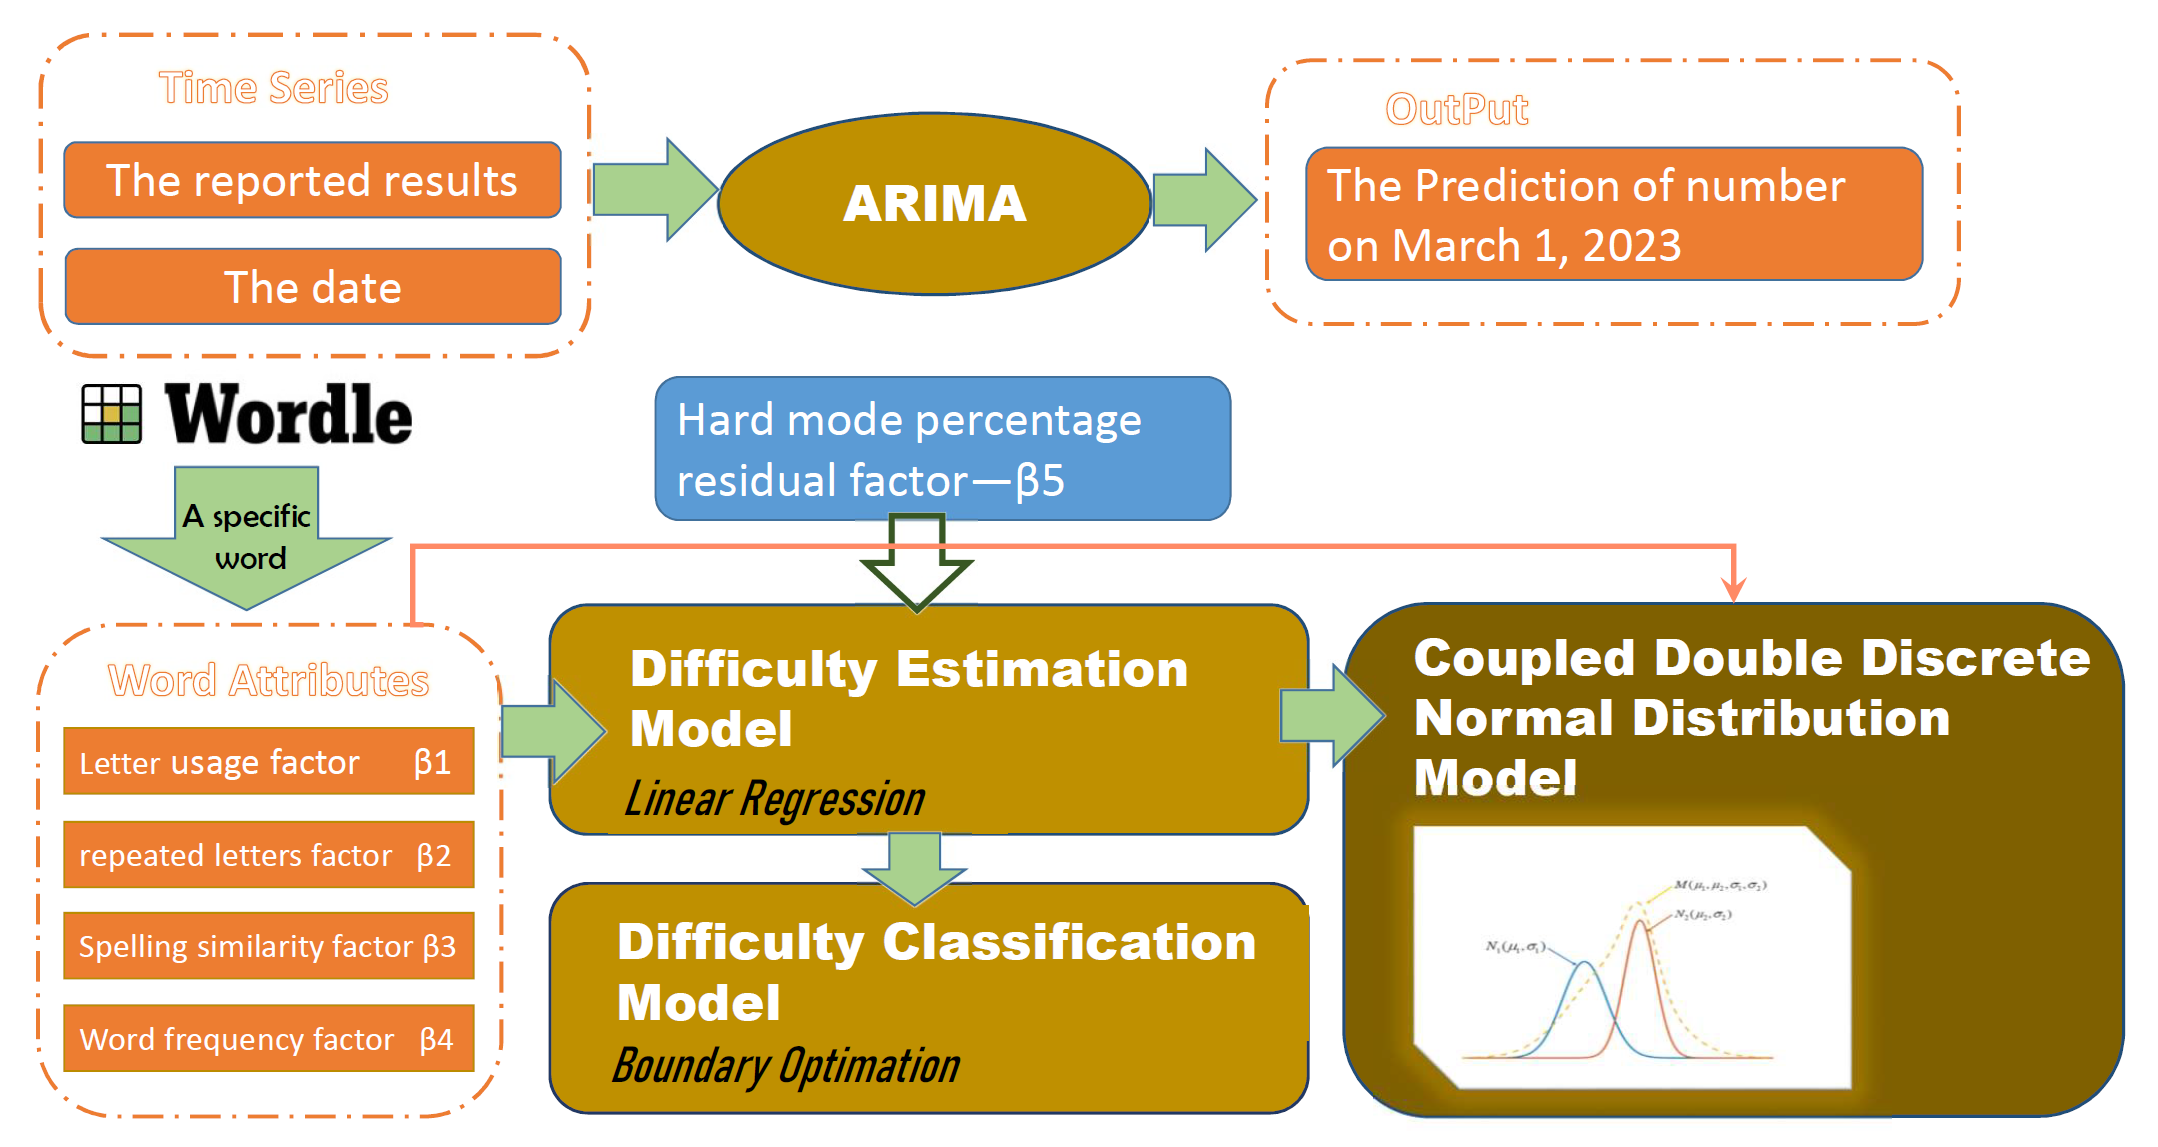
\includegraphics[height=0.5\textwidth]{overview}
\end{figure}
\section{Assumptions and Justifcations}
\begin{itemize}
\item \textbf{No major events related to wordle games happen during the time predicted by the model, which means the change of wordle games' popularity is stable:} The occurrence of major events can cause unanticipated changes in the number of users of wordle games, which greatly affects the model accuracy.
\item \textbf{Player proficiency variation affects the distribution of the reported results, and thus the difficulty is affected to a greater extent.:} There is a certain regularity in the change of proficiency of the player community for wordle games, which means no particularly effective wordle cheats have emerged
\item \textbf{The data is reported as true, and the reported players are not special, which means the data obtained is true and valid:} Reporting data that is true or from a particular group, such as professional gamers or bots, increases the uncertainty significantly and produces results that are not applicable to the general public. 
\end{itemize}
\section{Notations}
\begin{table}[!htbp]
	\small
	\centering
	\captionsetup{font={small}} 
	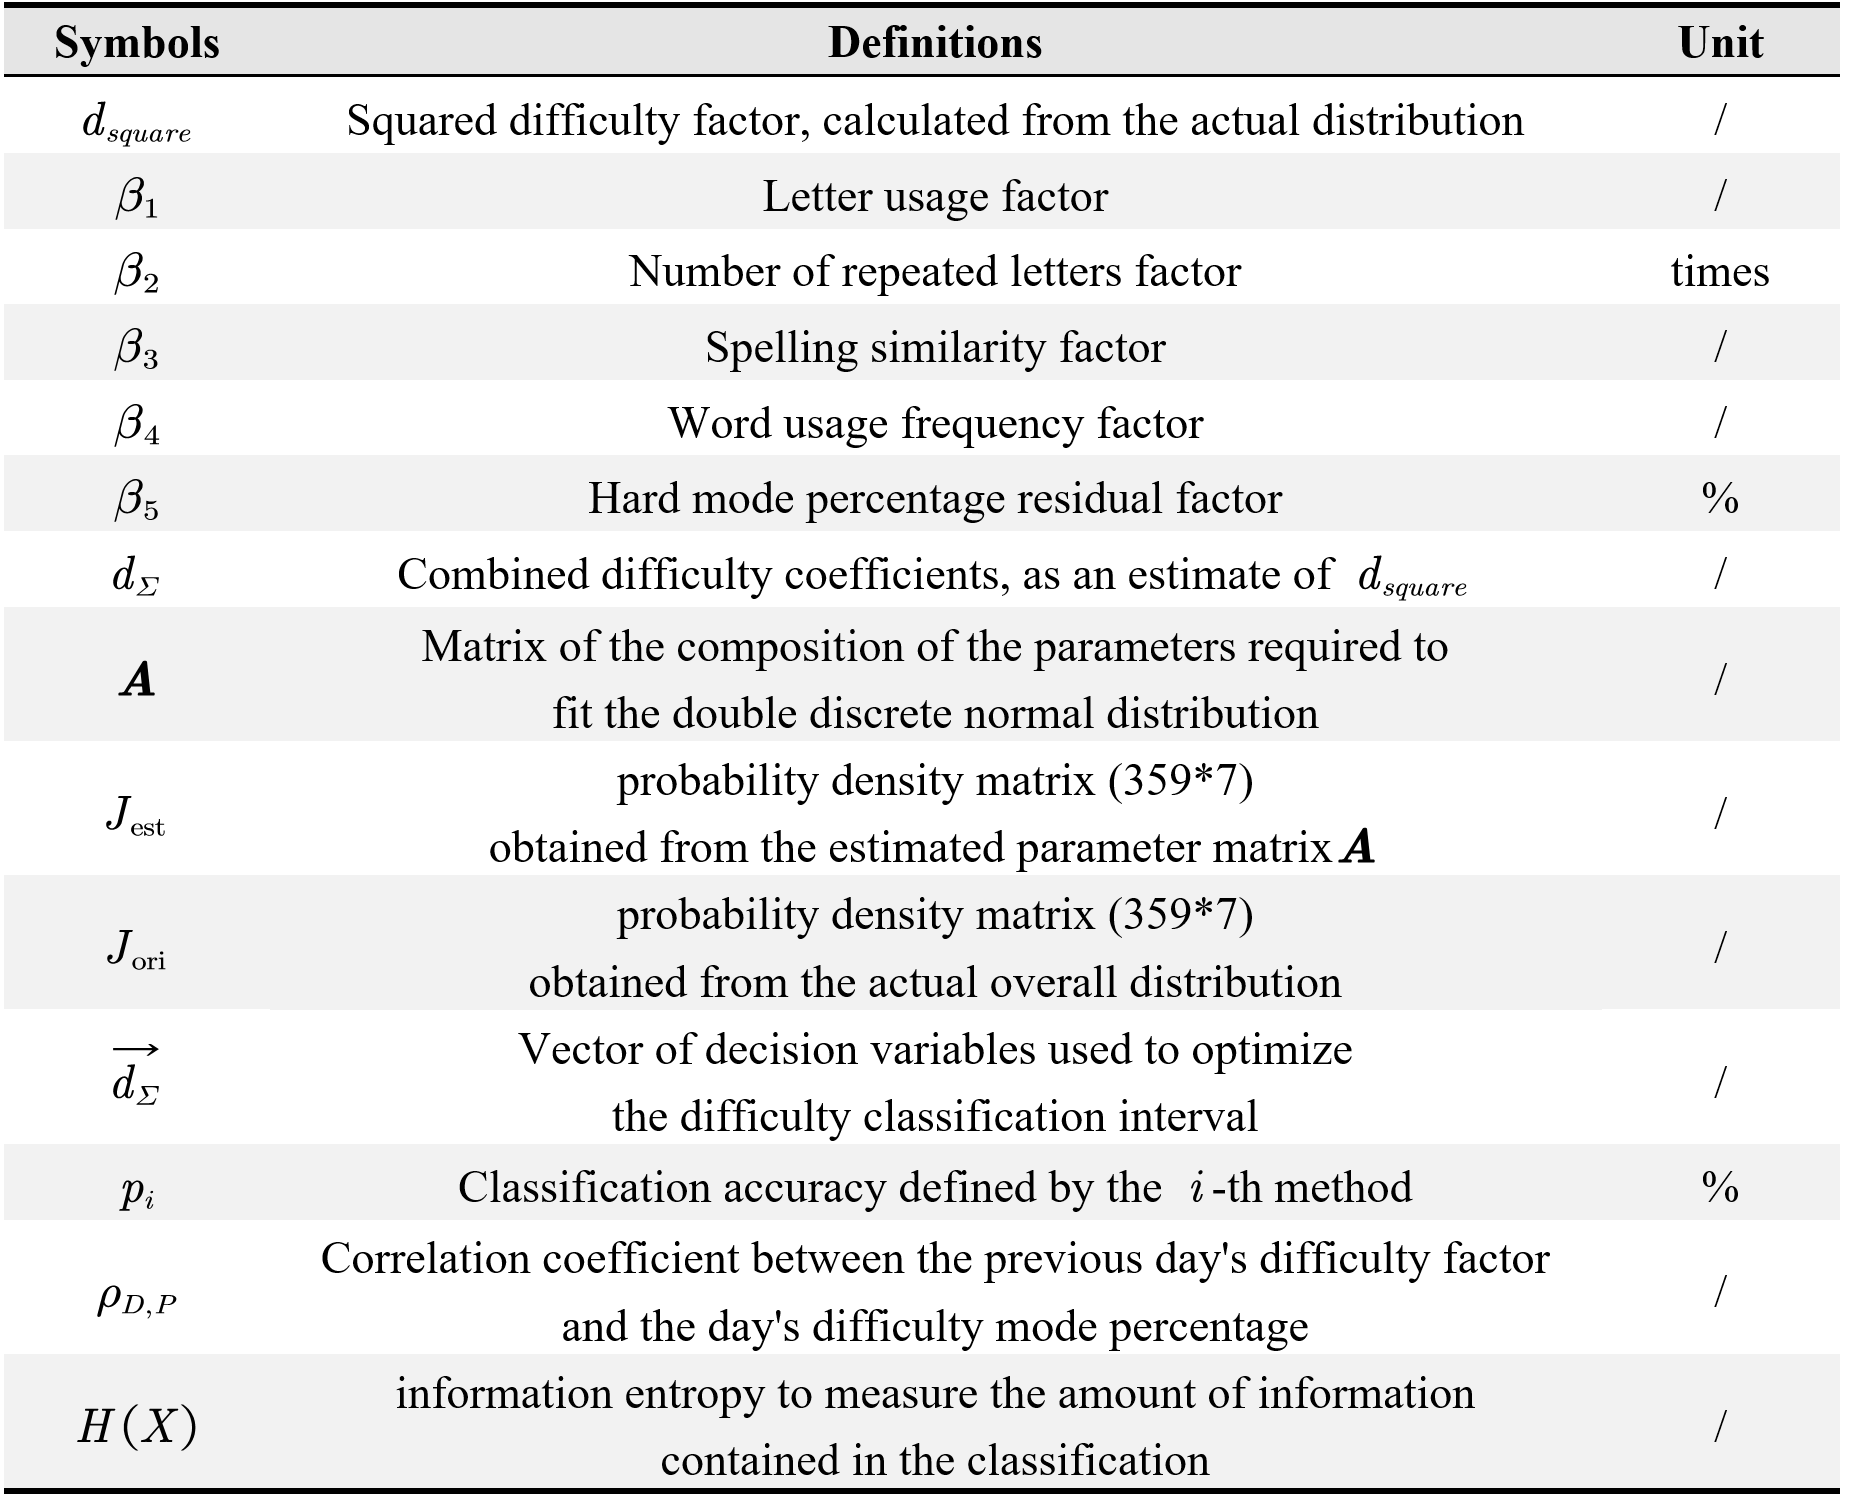
\includegraphics[height=0.8\textwidth]{notations}
\end{table}
\newpage
\section{ARIMA Time Series Prediction Model}
\subsection{Data Pre-processing of Daily Results}
\hspace{1.4em}First, we review the daily results file given in the title. The following errors are corrected:

\textbf{(a)} The total number of results reported on the day 2022/11/30 is 2596, an order of magnitude error, which we change to 25960.

\textbf{(b)} The solution words "clen" ,"marxh" and "tash" for the days 2022/11/26, 2022/10/5 and 2022/4/29 do not exist and should be "clean ", "marsh" and "trash".

Next, we find that the number of results reported is time series data in days. We want to predict the data at some future time points from the existing time series.

Considering that linearly varying time series are easier to handle, linearization of the raw data is required. Figure \ref{fig:2}(a) gives the original time series in the order of content number, and it can be found that the second half of the curve is roughly decreasing exponentially. Figure \ref{fig:2}(b) can be obtained by taking the logarithm.
\begin{figure}[h]
	\centering
	\captionsetup{font={small}}
	\begin{minipage}[c]{0.48\textwidth}
		\centering
		\includegraphics[width=\textwidth]{n}
		\subcaption{The original time series varies exponentially}
		\label{fig2_1}
	\end{minipage}
	\begin{minipage}[c]{0.49\textwidth}
		\centering
		\includegraphics[width=\textwidth]{ln(n)}
		\subcaption{The processed time series varies linearly}
		\label{fig2_2}
	\end{minipage}
	\caption{Trend analysis of "Number of reported result"}
	\label{fig:2}
\end{figure}

From the above figure, we can see that the logarithm of the Number of reported result changes roughly linearly after the Contest number reaches 350 days.
\\[0.01pt]
\subsection{Type Determination of ARIMA (p,d,q)}
\hspace{1.4em}For a linearly varying non-stationary time series, it can be analyzed using the ARIMA model, which transforms the non-stationary time series into a stationary time series and then regresses the dependent variable only on its lagged values and the present and lagged values of the random error term\cite{1}. It can be used to predict data for future periods based on historical data. 

Before using the ARIMA model, it is necessary to determine its type parameters $ (p, d, q) $, where $ p $ is the number of autoregressive terms, $ q $ is the number of sliding average terms, and $ d $ is the number of differences (orders) made to make it a smooth series. The type is determined based on the following steps.

\textbf{(1)Time series smoothness test}

It is not difficult to find that the number of people playing wordle shows a trend of first surge and then slow decline, possibly because the game was very popular when it was first launched, and as time goes by people's enthusiasm for wordle is gradually fading. And the ARIMA model is used to predict the time-series data, which must be stable. So in the subsequent prediction, we only use the data starting from 2022/6/4 to ensure the accuracy of the model.
\begin{table}[!htbp]
	\small
	\centering
	\captionsetup{font={small}} 
	\caption{ADF Checklist}
	\includegraphics[height=0.19\textwidth]{table1}
	\label{tab:1}
\end{table}

We perform a smoothness test on the second half of the intercepted time series\cite{2}. According to the results of ADF test (Augmented Dickey-Fuller test) in table\ref{tab:1}, the significance p-value is 0.000***(Significance level, *** represents error rate<1\%) at the level of significance when the difference is divided into 1st or 2nd order, the original hypothesis is rejected and the series is a smooth time series.

\textbf{(2)Estimation of p and q values based on truncated tails}

ACF (autocorrelation analysis) and PACF (partial autocorrelation analysis) were performed on the time series and the results are as follows.
\begin{figure}[h]
	\centering
	\captionsetup{font={small}}
	\begin{minipage}[c]{0.48\textwidth}
		\centering
		\includegraphics[width=\textwidth]{acf}
		\subcaption{ACF}
		\label{fig3_1}
	\end{minipage}
	\begin{minipage}[c]{0.48\textwidth}
		\centering
		\includegraphics[width=\textwidth]{pacf}
		\subcaption{PACF}
		\label{fig3_2}
	\end{minipage}
	\caption{Autocorrelation and partial autocorrelation plots of the final differential data}
	\label{fig:3}
\end{figure}

Figure \ref{fig:3} shows the differential data autocorrelation plot (ACF) and partial autocorrelation plot (PACF), including coefficients, upper confidence limits and lower confidence limits. It can be seen where the ACF plot is truncated and the PACF plot is trailed.

Based on the AIC information criterion to calculate the optimal parameters, the model results in an ARIMA model (1,1,1), while the goodness-of-fit $ R^{2} $ of the model is 0.947, which can basically meet the requirements. The model equation is given as follows:
\begin{equation}\label{eq:1}
u\left( t \right) =-0.005+0.193*u\left( t-1 \right) -0.859*\varepsilon \left( t-1 \right) 
\end{equation}
where $ u(t) $ is the first-order difference term and $ \varepsilon (t) $ is the noise difference term, we have:
\begin{equation*}\label{}
\begin{aligned}
	&y\left( t \right) =\ln \left( \text{Number\ of\ reported\ result} \right)\\
	&u\left( t \right) =y\left( t \right) -y\left( t-1 \right) 
\end{aligned}
\end{equation*}
\\[0.01pt]
\subsection{Model Solving}
\subsubsection{Interval forecast of the number of results on March 1, 2023}
\hspace{1.4em}Inputting the linearized data into the ARIMA model and taking the exponential operation on the results leads to the prediction results in the following figure,
\begin{figure}[h]
	\centering
	\captionsetup{font={small}}
	\begin{minipage}[c]{0.56\textwidth}
		\centering
		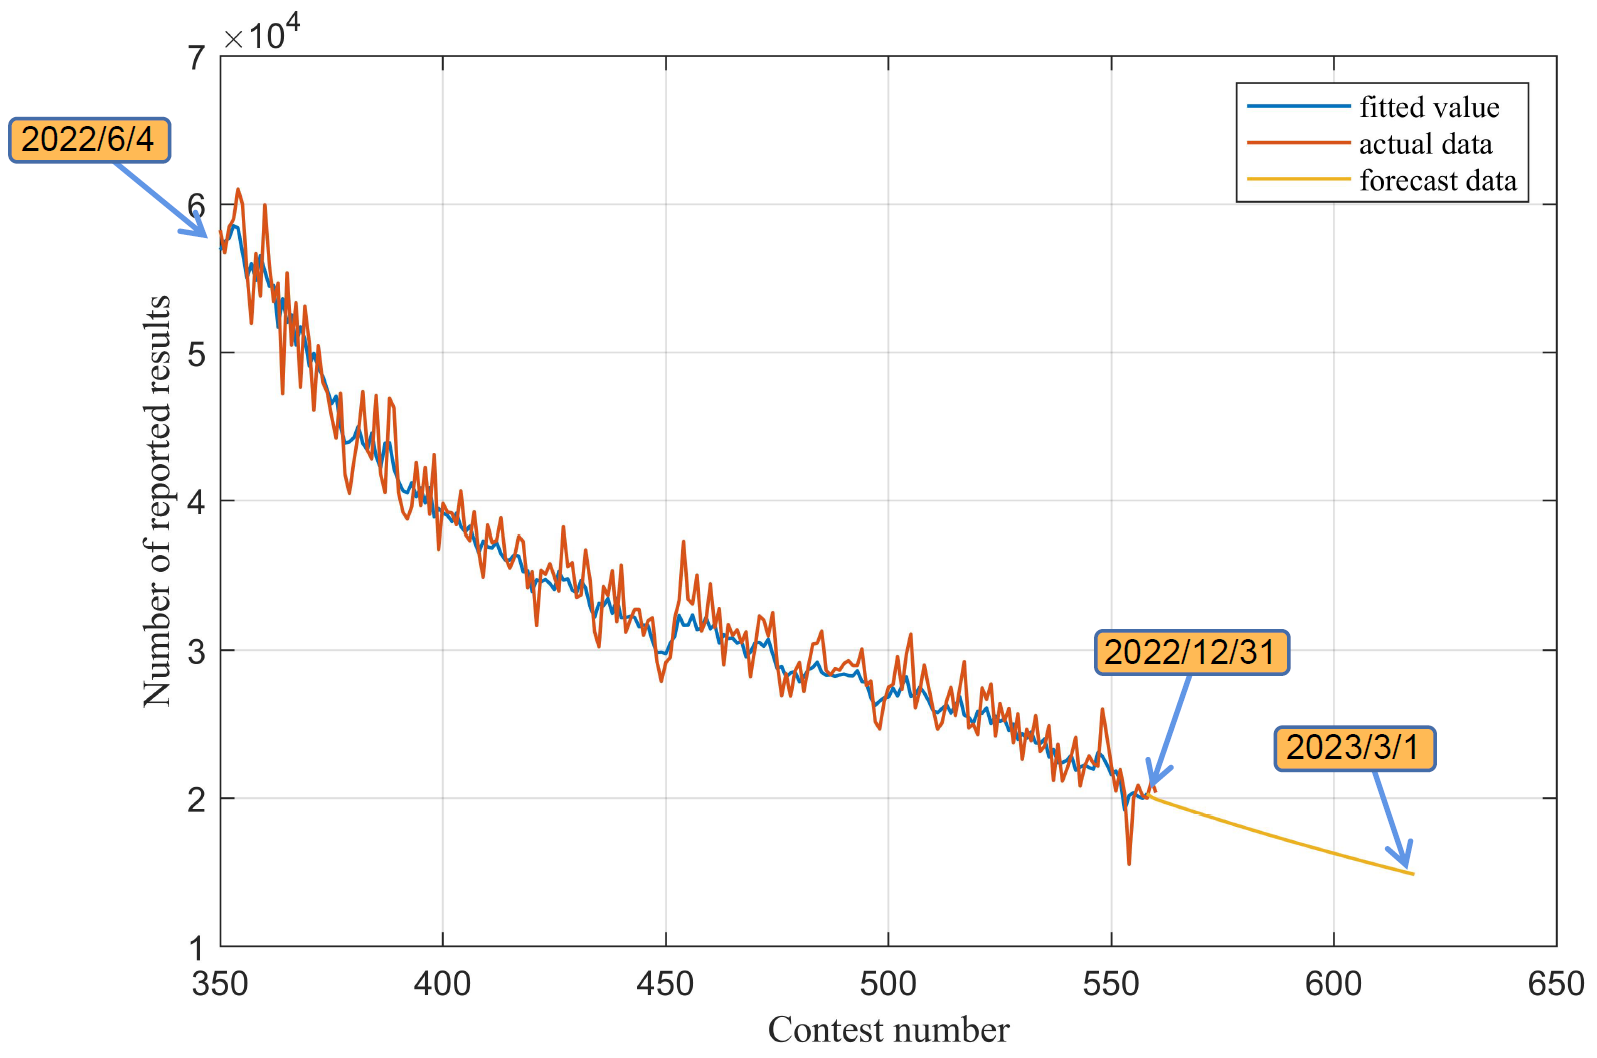
\includegraphics[width=\textwidth]{num}
		\label{fig4_1}
	\end{minipage}
\quad
	\begin{minipage}[c]{0.4\textwidth}
		\centering
		\includegraphics[width=\textwidth]{table2}
		\label{fig4_2}
	\end{minipage}
	\caption{Autocorrelation and partial autocorrelation plots of the final differential data}
	\label{fig:4}
\end{figure}
where the red line represents the true value provided by the question, the blue line represents the fitted value calculated according to equation 1, and the yellow line represents the predicted value. It can be seen that the predicted results obtained by the model show a smooth downward trend from the beginning of 2023 until March 1. It shows that the heat of wordle is still decaying slowly, maintaining the long trend since 2022/6/4(contest number=350). This also shows that the prediction result of our model is reasonable.

The Table above shows the number of Reported Results as of March 1, 2023, as projected by the ARIMA model. To obtain the prediction interval for the number of outcomes, we calculate the variance, which is $ \sigma^{2}=0.005694239 $ and the standard deviation obtained by extracting square root is $ \sigma=0.075460179 $. Substituting $ y = 14868.61498 (\ln y = 9.607008196) $, we can obtain $ \ln y = 9.60700819 \pm  0.075460179 $. It can be found that the interval of the number of reported outcomes at 2023/3/1 is

\begin{equation}\label{eq:2}
	y = [ 13787.91843,16034.02601 ]
\end{equation}
\\[0.01pt]
\subsubsection{The effect of word attributes on the choice of hard mode}
\hspace{1.4em}The attributes of words have almost no effect on the percentage in hard mode, since no one knows what the word of the day is until he or she play wordle, and the only accident where the percentage in hard mode can be affected by words may be giving up the game because it is too difficult, or being influenced by friends who have already played today, and the probability of this happening is very small. This can also be seen in the data. Let's roughly summarize the difficulty of each word for now as follows.

For the solution words on a given day, assuming that the percentage of passes after $ i $ attempts is $ \alpha_{i} $, we can define the square difficulty factor $ d_{square} $ of the vocabulary for that day as:

\begin{equation}\label{eq:3}
d_{square}=\dfrac{\sum_{i=1}^7{i^{2}\cdot \alpha _{i}}}{1^{2}+2^{2}+...+7^{2}}
\end{equation}

The daily data were sorted in descending order according to their square difficulty factor $ d_{square} $, and the days with higher difficulty factors were taken out to calculate their percentage of people who chose hard mode as shown in Table \ref{tab:3}. It can be found that the percentage of those days with similar and higher difficulty factors are not usually equally high in the hard mode. There are lower values such as 2.8$ \% $ and 4.0$ \% $. This indicates that the attributes of the words do not affect the percentage of players who choose the hard mode.
\begin{table}[!htbp]
	\small
	\centering
	\captionsetup{font={small}} 
	\caption{Listed in descending order of square difficulty factor $ d $}
	\includegraphics[height=0.128\textwidth]{table3}
	\label{tab:3}
\end{table}
\begin{table}[!htbp]
	\small
	\centering
	\captionsetup{font={small}} 
	\caption{Listed in descending order by the percentage of people who chose hard mode}
	\includegraphics[height=0.128\textwidth]{table4}
	\label{tab:4}
\end{table}

In contrast, if we take the percentage of people choosing the hard mode in descending order and calculate its square difficulty factor $ d_{square} $, we can find that the two show a positive correlation at this point, as shown in Table \ref{tab:4}. This suggests that it is not the attributes of the words that are influencing the players' mode choice. Rather, players' mode choices affect the square difficulty factor $ d_{square} $ of the words. This is because when the proportion of people choosing the hard mode increases, the situation of the number of answers of the day is affected by it, resulting in a higher overall difficulty factor.

In summary, it can be seen that the proportion of people choosing the hard mode is largely unaffected by the word attributes of the day. However, it is possible that the attributes of words have different effects on the distribution of attempts in different ways, which we will analyze in detail later.
\\[0.01pt]
\section{Difficulty Evaluation Model Based on Word Attributes}
\subsection{Analysis of Word Attributes}
\hspace{1.4em}In 4.3.2, we have determined a square difficulty factor $ d_{square} $ for the word of the day based on the distribution data of the number of attempts, and this method is quite convenient and accurate. However, if we want to calculate the difficulty of words only from the words themselves, we need to determine some attributes of the words that are closely related to their difficulty(We only choose word attributes that are typical and correlate well with difficulty):

\textbf{a)} \textit{Letter usage factor}---$ \beta_{1} $

Among the 26 letters of the alphabet, the probability of different letters appearing in words and the usage frequency in people's daily life are different\cite{3}. For the more commonly used letters, people will use them more frequently when playing wordle, and thus words containing these letters will be more easily guessed. The letter usage factors is defined as follows:

\begin{equation}\label{eq:10}
\beta _1=\sum_{i=1}^5{u_i\times 100}
\end{equation}

The $ u_{i} $ in Equation \ref{eq:10} indicates the usage frequency of the i-th letter of the 5 letters of the solution word.

\textbf{b)} \textit{Number of repeated letters}---$ \beta_{2} $

When there are multiple repeated letters in a word, it is often more difficult to guess at that point. This is because during the wordle game, when people guess a letter in a word, they are more inclined to think about whether there are other letters in the word, which makes it difficult to guess words with more than one repeated letter. The number of repeated letters factor is defined as follows:

\begin{equation}\label{eq:11}
\beta _2=N_{\text{repeated}}^{r_{1}}
\end{equation}

$ N_{\text{repeated}} $ in equation \ref{eq:11} is the number of repeated occurrences of the same letter in the word, and after calculating the correlation coefficient between this factor and the square difficulty factor $ d_{square} $, the final $ r_{1}=1.3 $ was taken.
\begin{figure}[h]
	\centering
	\captionsetup{font={small}}
	\begin{minipage}[c]{0.45\textwidth}
		\centering
		\includegraphics[width=\textwidth]{word1}
		\subcaption{Number of repeated letters}
		\label{fig9_1}
	\end{minipage}
	\begin{minipage}[c]{0.5\textwidth}
		\centering
		\includegraphics[width=\textwidth]{word2}
		\subcaption{Spelling similarity factor}
		\label{fig9_2}
	\end{minipage}
	\caption{An example of how the word attribute factor is calculated}
	\label{fig:9}
\end{figure}

\textbf{c)} \textit{Spelling similarity factor}---$ \beta_{3} $

If a word has many words with similar spellings, it can be difficult for people to guess it from the wordle's alphabetic cues. This is because when people type in the word that is similar to it and the system declares a mistake, they may go on to think of other words. We define the spelling similarity factor as:

\begin{equation}\label{eq:12}
\beta _3=e^{r_2\cdot n}
\end{equation}

In Equation \ref{eq:12}, $ n $ is the number of words with similar spellings to the word(5 letter words that differ by only 1 letter), and after calculating the correlation coefficient between this factor and the square difficulty factor, $ r_{2} $ is determined to be 0.18.

\textbf{d)} \textit{Word usage frequency factor}---$ \beta_{4} $

The word usage frequency directly affects the likelihood of people guessing the word. For words that people use frequently, it is much easier to guess it. There is a strong correlation between the frequency of word use and the difficulty of wordle puzzles. We define the word usage frequency factor\cite{4} as:

\begin{equation}\label{eq:13}
\beta _4=\left( \ln f \right) ^{r_3}
\end{equation}

Where $ f $ in Equation \ref{eq:13} is the relative frequency of word usage. After calculating the correlation coefficient between the current factor and the square difficulty factor, $ r_{3} $ is taken to be 0.3.

\textbf{e)} \textit{Hard mode percentage residual factor}---$ \beta_{5} $

The square difficulty factor $ d_{square} $ is influenced to some extent by the percentage of hard mode selected, which increases with time in a somewhat regular manner, but the difficulty factor is stable. In order to separate the relationship between the two, we chose to fit the trend of the percentage change of hard mode by the inverse tangent function first, and then analyze the relationship between the residuals and the difficulty factor\cite{5}. The functions used for the fitting are as follows, and Figure \ref{fig:10}(a) illustrates the good results of the fitting.

\begin{equation}\label{eq:16}
\bar{z}=0.0679\times \arctan \left( 0.01n+0.1 \right) +0.0094
\end{equation}

In Equation \ref{eq:16} $ \bar{z} $ is an estimate of the percentage of difficulty mode, corresponding to $ z $ as the true value. Using the residuals $ e $ as a new attribute of word, the hard mode percentage residual factor can be defined as follows:
\begin{equation}\label{eq:17}
	\begin{aligned}
		\beta _5=e&=z-\bar{z}\\
		&=z-0.0679\times \arctan \left( 0.01n+0.1 \right) +0.0094
	\end{aligned}
\end{equation}
\\[0.01pt]
\subsection{Model Solving}
\begin{figure}[h]
	\centering
	\captionsetup{font={small}}
	\begin{minipage}[c]{0.34\textwidth}
		\centering
		\includegraphics[width=\textwidth]{5-1}
		\subcaption{Fitting results for the percentage of hard mode}
		\label{fig10_1}
	\end{minipage}
	\begin{minipage}[c]{0.65\textwidth}
		\centering
		\includegraphics[width=\textwidth]{5-2}
		\subcaption{The estimated results of $ d_{\varSigma} $ on $ d_{square} $}
		\label{fig10_2}
	\end{minipage}
	\caption{Determination of the parameters of the word difficulty evaluation model}
	\label{fig:10}
\end{figure}
We consider the square difficulty factor $ d_{square} $ calculated from the true distribution data to be plausible, and therefore make it the dependent variable, and then perform a stepwise linear regression with each of our selected factors, $ \beta_{2} $, as the independent variable. We expect to be able to explain the difficulty of words in terms of these word attributes, and the results is:

\begin{equation}\label{eq:14}
d_{\varSigma}=-0.097\beta _1+1.569\beta _2+0.151\beta _3-3.701\beta _4+180.892\beta _5+22.618
\end{equation}

In equation 8 $ d_{\varSigma} $ is the estimated value of $ d_{square} $, which we will refer to later as the combined difficulty factor, representing that this difficulty factor is calculated from each attribute of the word only. We can also see from equation that the coefficients of $ \beta_{1} $ and $ \beta_{2} $ are negative, indicating that more frequent use of the word or more frequent use of letters in the word leads to a decrease in the overall difficulty of the word. The coefficients of $ \beta_{3} $ and $ \beta_{4} $ are positive, indicating that more repetitions of letters in the word or more words similar to the word leads to an increase in the overall difficulty of the word. These phenomena are all consistent with common sense and suggest that our model for evaluating difficulty is reasonable.

From the above graph we can see that on the vast majority of the 359 days, the combined difficulty factor $ d_{\varSigma} $ (estimated) is closer to the square difficulty factor $ d_{square} $ (actual). A significant difference between the two in some days can be explained by the fact that the distribution of these days is influenced not only by the attributes of the words themselves, but also by certain external factors, such as Internet trends, hot events, etc.
\\[0.01pt]
\section{Coupled Double Discrete Normal Distribution Fitting Model}
\subsection{Normal Distribution Decomposition of the Overall Distribution}
\subsubsection{Inference of overall distribution form}
\hspace{1.4em}We all know that the distribution of all students' scores in a test can be approximated by a normal distribution. Similarly, a similar pattern should be found in wordle, which has a larger sample size.

\begin{figure}[h]
	\small
	\centering
	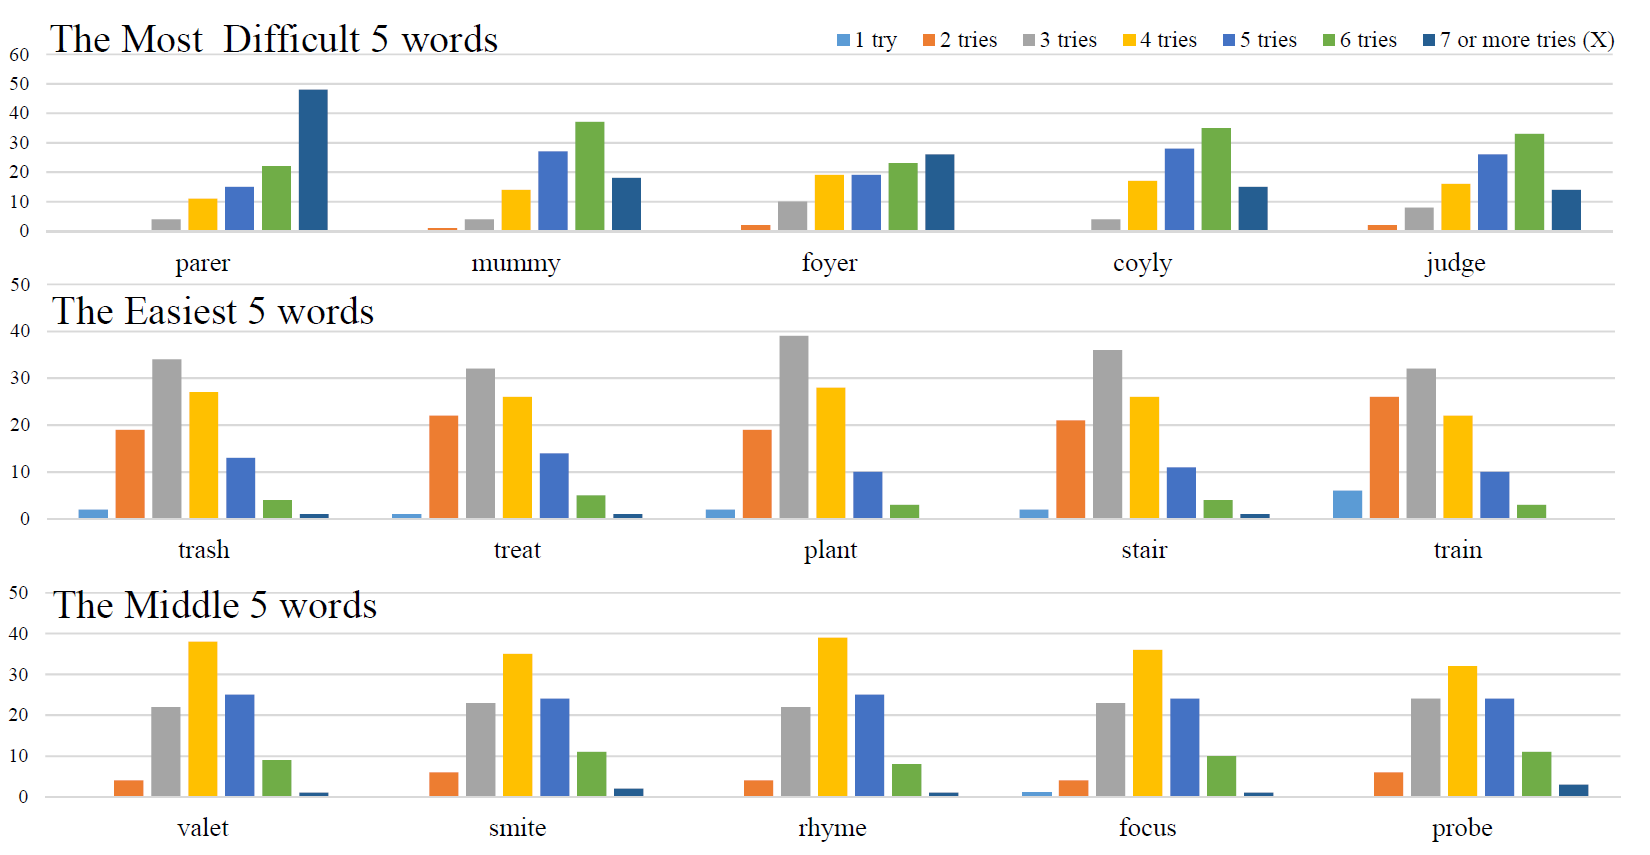
\includegraphics[height=0.53\textwidth]{15}
	\captionsetup{font={small}}
	\caption{Effect of word attributes (e.g., $ d_{\varSigma } $) on the overall report distribution} 
	\label{fig:6}
\end{figure}
It is observed in the data that the percentages that people report show some degree of normal distribution, but do not exactly fit the normal distribution. According to the difficulty evaluation method in the previous section, the standard deviation of the number of attempts reported when the combined difficulty factor $ d_{\varSigma } $ is high are larger than those lower, as shown in Figure \ref{fig:6}. Accordingly, we hypothesize that the overall distribution of reports will be influenced by certain attributes of the words and show some normality.

Given the observed phenomena and the above inferences, we believe that the distribution of reported results should be influenced by the combined difficulty factor and certain characteristics of the words. People's word-guessing results in wordle tournaments should also obey a normal distribution, but in the sample of statistics, the tournament results of players playing the hard mode and the normal mode were not counted separately, which led to some deviations from the expected statistical results.

\begin{wrapfigure}{r}{10cm}
	\small
	\centering
	\includegraphics[width=0.52\textwidth]{normal1}
	\captionsetup{font={small}}
	\caption{Two normal distribution probability density synthesis} 
	\label{fig:5}
\end{wrapfigure}
The reason for this phenomenon may be that the distribution of the reported results in normal mode is different from that of the reported results in hard mode. Nevertheless, we can still assume that the reported results in the normal mode and the reported results in the hard mode both obey a normal distribution. On this basis, it is reasonable to infer that the PDF of the overall distribution of the number of attempts is a combination of the PDFs of the normal and difficult modes, as shown in Figure \ref{fig:5}. This combination can be viewed simply as a linear combination, i.e., a weighted sum. The overall (mixed normal and hard mode) reported outcomes $ X $ obey the following distribution $ M $, $ M $ is a combination of the normal distribution $ N_{1} $ for the normal mode reported results and the normal distribution $ N_{2} $ for the hard mode reported results:

\begin{equation}\label{eq:4}
X\sim M\left( \mu _1,\sigma _1,\mu _2,\sigma _2 \right)
\end{equation}

where $ \mu _1,\sigma _1 $ and $ \mu _2,\sigma _2 $ are from $ N_{1}(\mu _1,\sigma _1) $ and $ N_{2}(\mu _2,\sigma _2) $, respectively, and are the means and standard deviations of two normal distributions for the normal and hard mode.
\\[0.01pt]
\subsubsection{Determination of model parameters}
\hspace{1.4em}For different solution words, the distribution of the number of attempts should also be different for the normal and hard modes, so the parameters of the normal distribution - the mean and standard deviation - should be closely related to the properties of the words. The combined difficulty factor $ d_{\varSigma } $ we obtained in the previous section can be an important basis for determining $ \mu _1,\mu _2,\sigma _1,\sigma _2 $, but difficulty alone does not provide a good description of a word's attributes. For this reason, we introduce the most representative word attribute in 5.1, Number of repeated times $\beta_2$, as an additional parameter that jointly determines the distribution $ M $ with $ d_{\varSigma } $. Arguing that the parameters of $ N_{1},N_{2} $ should be determined jointly by $ d_{\varSigma } $ and $\beta_2$, and that one of the simplest ways to determine the parameters is to consider them to be linearly related:

\begin{equation}\label{eq:5}
	\left\{\begin{array}{l}
		\mu_1=k_1\cdot d_{\varSigma }\left(\beta_1, \beta_2, \cdots,\beta_5\right)+w_{1} \beta_2+b_1 \\
		\mu_2=k_2\cdot d_{\varSigma }\left(\beta_1, \beta_2, \cdots,\beta_5\right)+w_{2} \beta_2 +b_2 \\
		\sigma_1=k_3\cdot d_{\varSigma }\left(\beta_1, \beta_2, \cdots,\beta_5\right)+w_{3} \beta_2+b_3 \\
		\sigma_2=k_4\cdot d_{\varSigma }\left(\beta_1, \beta_2, \cdots,\beta_5\right)+w_{4} \beta_2+b_4 
	\end{array}\right.
\end{equation}

When the solution word of the day is determined, its various attributes indicators $\beta_2$ and the combined difficulty factor $ d_{\varSigma }\left(\beta_1, \beta_2, \cdots,\beta_5\right) $ can be uniquely determined, we denote the parameter matrix containing $ k_{i} $, $ w_{i} $, $ b_{i} $ to be solved as $ \boldsymbol{A} $.
\\[0.01pt]
\subsection{Model Optimization by Nonlinear Least Squares}
\hspace{1.4em}We split the reported overall number of attempts distribution of the PDF into a weighted sum of the normal distribution PDF for the normal mode and the normal distribution PDF for the difficult mode. Obviously these two distributions should be discrete and should satisfy the expression for the discrete normal distribution:

\begin{equation}\label{eq:7}
	P_i(X=x)=\dfrac{1}{\sqrt{2 \pi} \sigma_i} e^{\frac{-\left(x-\mu_i\right)^2}{2 \sigma_i^2}}(x=1,2, \cdots 7)
\end{equation}

In the above we assumed that the probability density of the overall distribution can be written as a weighted sum of the probability densities of the ordinary and hard modes. Then for a given day of solution words, the probability (percentage) of the number of guesses $ X=x $ for that day can be obtained as the weighted sum of the probability (percentage) of the number of guesses $ X_{1}=x $ and $ X_{2}=x  $ for both modes for that day:

\begin{equation}\label{eq:8}
P\left( X=x \right) =\alpha P_1\left( X_{1}=x \right) +\left( 1-\alpha \right) P_2\left( X_{2}=x \right) 
\end{equation}
where $ P $ is the probability of $ X $ taking different attempts in the overall number of attempts distribution $ M $, multiplied by 100\% is the percentage. $ \alpha $ is the percentage of the total number of people playing Normal mode, calculated as $ \alpha = 0.925 $ based on the mean value of the percentage in 359 statistics.

In order to estimate the parameter matrix $ \boldsymbol{A} $ constructed in Equation \ref{eq:6}, denote $ \boldsymbol{A} $ as the decision variable. It is necessary to find a suitable parameter matrix $ \boldsymbol{A} $ such that it determines two normal distributions. In turn, the most appropriate distribution prediction of the overall number of attempts is obtained from the predetermined weights.

We use a nonlinear least squares optimization method to compare the estimated overall number of attempts distribution with the actual distribution. In this way, the parameter matrix $ \boldsymbol{A} $ that brings the estimated distribution closest to the overall distribution is what we are looking for. Based on the above idea, the objective function $ G(d_{\varSigma }, \beta_2) $ can be constructed.

\begin{equation}\label{eq:9}
\begin{array}{r}
	\min G(d_{\varSigma }, \beta_2)=\left\|J_{\text {est}}-J_{\text {ori }}\right\|^2 ~\\
	\vspace{0.2em}\\
	J_{\text {est }}=100\% \times\left[\begin{array}{llll}
		P_{1,1} & P_{1,2} & \cdots & P_{1,7} \\
		P_{2,1} & P_{2,2} & \cdots & P_{2,7} \\
		\vdots & \vdots & \ddots & \vdots \\
		P_{359,1} & P_{359,2} & \cdots & P_{359,7}
	\end{array}\right]
\end{array}
\end{equation}

$ J_{\text {est }} $ in the above equation is the probability density matrix (359*7) obtained from the estimated parameter matrix $ \boldsymbol{A} $ and multiplied by 100\% to obtain the percentage matrix. $ J_{\text {ori }} $ is the probability density matrix (359*7) obtained from the actual overall distribution of the number of attempts.
\begin{itemize}
	\item The goal of optimization is to minimize the $ \left\|J_{\text {est}}-J_{\text {ori }}\right\|^2 $ parameter, i.e., the least squares idea, and find the parameter matrix $ \boldsymbol{A} $ that minimizes $ G(d_{\varSigma },\beta_1, \beta_2, \cdots,\beta_p) $
	\item The optimization process is unconstrained optimization without setting constraints
	\item It is observed that the mean of the distribution of the hard model is generally larger than that of the normal model, which provides guidance for the setting of the initial values of the optimization process.
\end{itemize}
\subsection{Model Solving}
\subsubsection{Normal distribution fitting results}
\hspace{1.4em}The parameter matrix $ \boldsymbol{A} $ is obtained by optimal solution as follows:
\begin{equation}\label{eq:6}
	\boldsymbol{A}=\left[\begin{array}{lllll}
		k_1 & w_{1} & b_1  \\
		k_2 & w_{2} & b_2 \\
		k_3 & w_{3} & b_3 \\
		k_4 & w_{4} & b_4
	\end{array}\right]
=
\left[ \begin{matrix}
	0.1841&		0.0079&		1.6461\\
	0.1852&		364.33&		2.0331\\
	0.0337&		0.0784&		0.6579\\
	-258.51&		-1162.4&		2812.6\\
\end{matrix} \right] 
\end{equation}
At this point we can find out the normal distribution of the number of attempts in normal mode and hard mode only by each attribute of the word, and then synthesize to get the overall distribution, the effect of the fit is shown in Figure \ref{fig:7}.

The residuals between the fitted and actual results of the coupled double normal distribution for days 1-359 are shown in Figure \ref{fig:7}(a). The residuals are defined as shown in the figure, and it can be seen that only a few number of days have higher residuals. The distribution predictions for several words of different difficulty are shown in Figure \ref{fig:7}(b), and it can be seen that the model has good fitting results for words with large differences in attributes.
\begin{figure}[h]
	\centering
	\captionsetup{font={small}}
	\begin{minipage}[c]{1\textwidth}
		\centering
		\includegraphics[width=\textwidth]{error}
		\subcaption{Error of the model at different dates}
		\label{fig7_1}
	\end{minipage}
	\begin{minipage}[c]{0.52\textwidth}
		\centering
		\includegraphics[width=\textwidth]{7.2-1}
		\subcaption{Comparison of the distribution}
		\label{fig7_2}
	\end{minipage}
	\begin{minipage}[c]{0.43\textwidth}
	\centering
	\includegraphics[width=\textwidth]{eerie}
	\subcaption{EERIE distribution forecast for March 1, 2023}
	\label{fig7_3}
\end{minipage}
	\caption{Coupled double-normal distribution fitting results}
	\label{fig:7}
\end{figure}

The distribution of the number of attempts on that day can be solved according to the difficulty and word attributes of EERIE, as shown in Figure \ref{fig:7}(c).
\\[0.01pt]
\subsubsection{Uncertainty factors and forecast credibility}
\hspace{1.4em}\textbf{(1)}\textit{Uncertainty factors}

\textbf{a) Impact of major events on the active user base: } The occurrence of major events related to wordle may change the number and overall level of the wordle user base significantly, resulting in an impact on the distribution of the reported results.

\textbf{b) Impact of time lapse on the model: } Over time, users' proficiency in wordle games and the emergence of new solution sets will have an impact on the coefficients and prediction results of the model, and the longer the time lapse, the greater the impact and the greater the prediction error of the existing model.

\textbf{c) Impact of hard mode: } The percentage of people who choose hard mode changes the error parameter in the model, which affects the model prediction, but the question does not provide that percentage.

\textbf{d) Impact of other characteristics of the word itself: } such as the region of origin, the category of the word (word nature, word meaning), the hotness (frequency of use) of other words similar to the word, etc.

\textbf{(2)}\textit{Forecast credibility}

The difficulty factors $ d_{\varSigma } $ entered in the EERIE prediction are from the difficulty evaluation model developed in section 5, in which there is a certain error in the estimation of the combined difficulty factors, and we need to jointly consider the errors of the current fitted model and the previous evaluation model when discussing the accuracy of the "EERIE" prediction.

First, we can calculate the probability that the estimated difficulty factor of "EERIE" falls within the upper and lower bound of 10\% of the true difficulty factor $ p_{a}=55.99\% $, and the interval range is $ [13.46, 16.45] $. The upper and lower bounds of the distribution estimation results can be obtained by substituting the upper and lower bounds of the interval into the current fitted model.

Then, based on the probability that the predicted percentage falls within the true percentage $ 2\sigma $(The standard deviation corresponding to the predicted distribution of each number of attempts) range in the current fitted model can be obtained as $ p_{b}$. Thus, the upper and lower bounds of the estimated results are extended by another $ 2\sigma $
, then $ p_a\times p_b $ is the probability of the distribution in this expanded interval computed from the given word attributes and their estimated difficulty.
\begin{figure}[h]
	\small
	\centering
	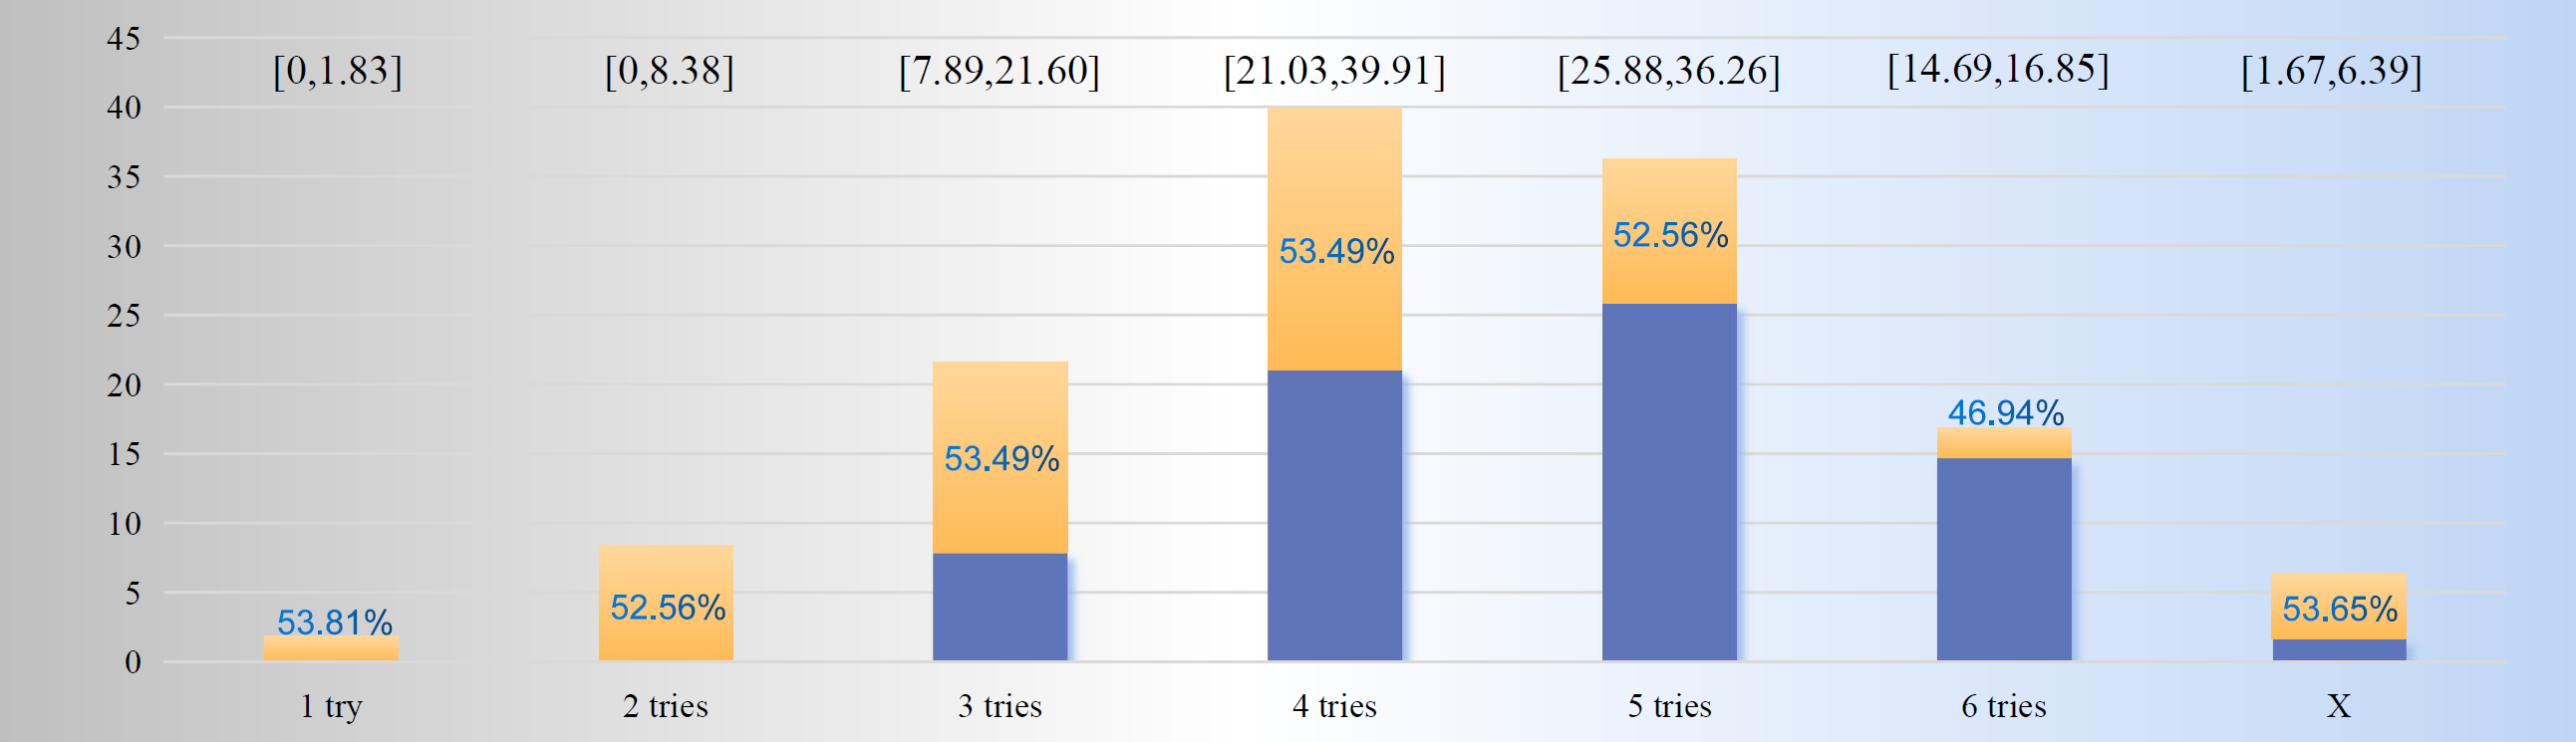
\includegraphics[height=0.29\textwidth]{conf}
	\captionsetup{font={small}}
	\caption{Confidence in EERIE distribution prediction} 
	\label{fig:15}
\end{figure}

Up to this point we quantified the confidence in the prediction, as shown in Figure \ref{fig:15}. For example, for the March 1 EERIE word, if the percentage of people attempting 3 times is regarded as the probability of $ [7.89,21.60] $, then we have at least 53.49\% confidence.
\\[0.01pt]
\section{Word Difficulty Classification Model Based on Boundary Optimization}
\subsection{Difficulty Classification Criteria}
\hspace{1.4em}The difficulty classification model is based on the difficulty evaluation model already given in section 5, and follows the word attribute metrics therein. The purpose of the classification is to determine a series of difficulty values that serve as boundaries for each class.
\begin{figure}[h]
	\small
	\centering
	\includegraphics[height=0.22\textwidth]{7.1-1}
	\captionsetup{font={small}}
	\caption{Classify words by difficulty stars} 
	\label{fig:13}
\end{figure}

If both the square difficulty factor $ d_{square} $ and the combined difficulty factor $ d_{\varSigma} $ of the same word fall in the same interval, the classification is considered correct, if $ d_{square} $ and $ d_{\varSigma} $ of the same word fall in different intervals, the classification is considered biased. The optimal classification interval can be searched by constructing the penalty function and developing an optimization strategy. Accordingly, if we need to divide the difficulty into four classes (i.e., three boundaries are needed), the decision variable can be determined as the value of the combined difficulty factor for the three boundary points: 

\begin{equation}\label{eq:18}
\vec{d}_{\varSigma}=\left[ d_{\varSigma 1},\ d_{\varSigma 2},\ d_{\varSigma 3}, \right]
\end{equation}

For the classification of difficulty level intervals, we expect that for a given identified word, its $ d_{square} $ and $ d_{\varSigma} $ fall in the same interval as far as possible, and the positions of $ d_{square} $ and $ d_{\varSigma} $ on the difficulty axes are as far as possible from the sides of the interval in which they are located. Following the above principles, the objective function shown in Figure \ref{fig:12} can be constructed.
\begin{figure}[h]
	\small
	\centering
	\includegraphics[height=0.3\textwidth]{7.1-2}
	\captionsetup{font={small}}
	\caption{Construction of the loss function} 
	\label{fig:12}
\end{figure}

Let the loss function be $ L(\vec{d}_{\varSigma}) $,$ d_{\varSigma} $ and $ d_{square} $ are known, and given the initial value, the optimal solution d is searched by the unconstrained optimization algorithm to obtain the optimal boundary for interval partitioning.
\\[0.01pt]
\subsection{Model Solving}
\subsubsection{How difficult is the word EERIE}
\hspace{1.4em}From the boundary optimization model constructed above, the difficulty boundary values are solved such that the combined difficulty factor $ d_{\varSigma} $ (estimated value) and the square difficulty factor $ d_{square} $ (plausible value) are assigned to the same category as far as possible. Finally we obtain that
$ 	\vec{d}_{\varSigma}=\left[  11.9558,\    13.6353,\    14.7029, \right] $.
By arranging all the words in descending order by $ d_{square} $, their combined difficulty factors are calculated according to Equation \ref{eq:14} and their difficulty stars can be obtained by dividing their categories according to the boundaries as shown in Figure \ref{fig:14}(b).
\begin{figure}[h]
	\centering
	\captionsetup{font={small}}
	\begin{minipage}[c]{0.26\textwidth}
		\centering
		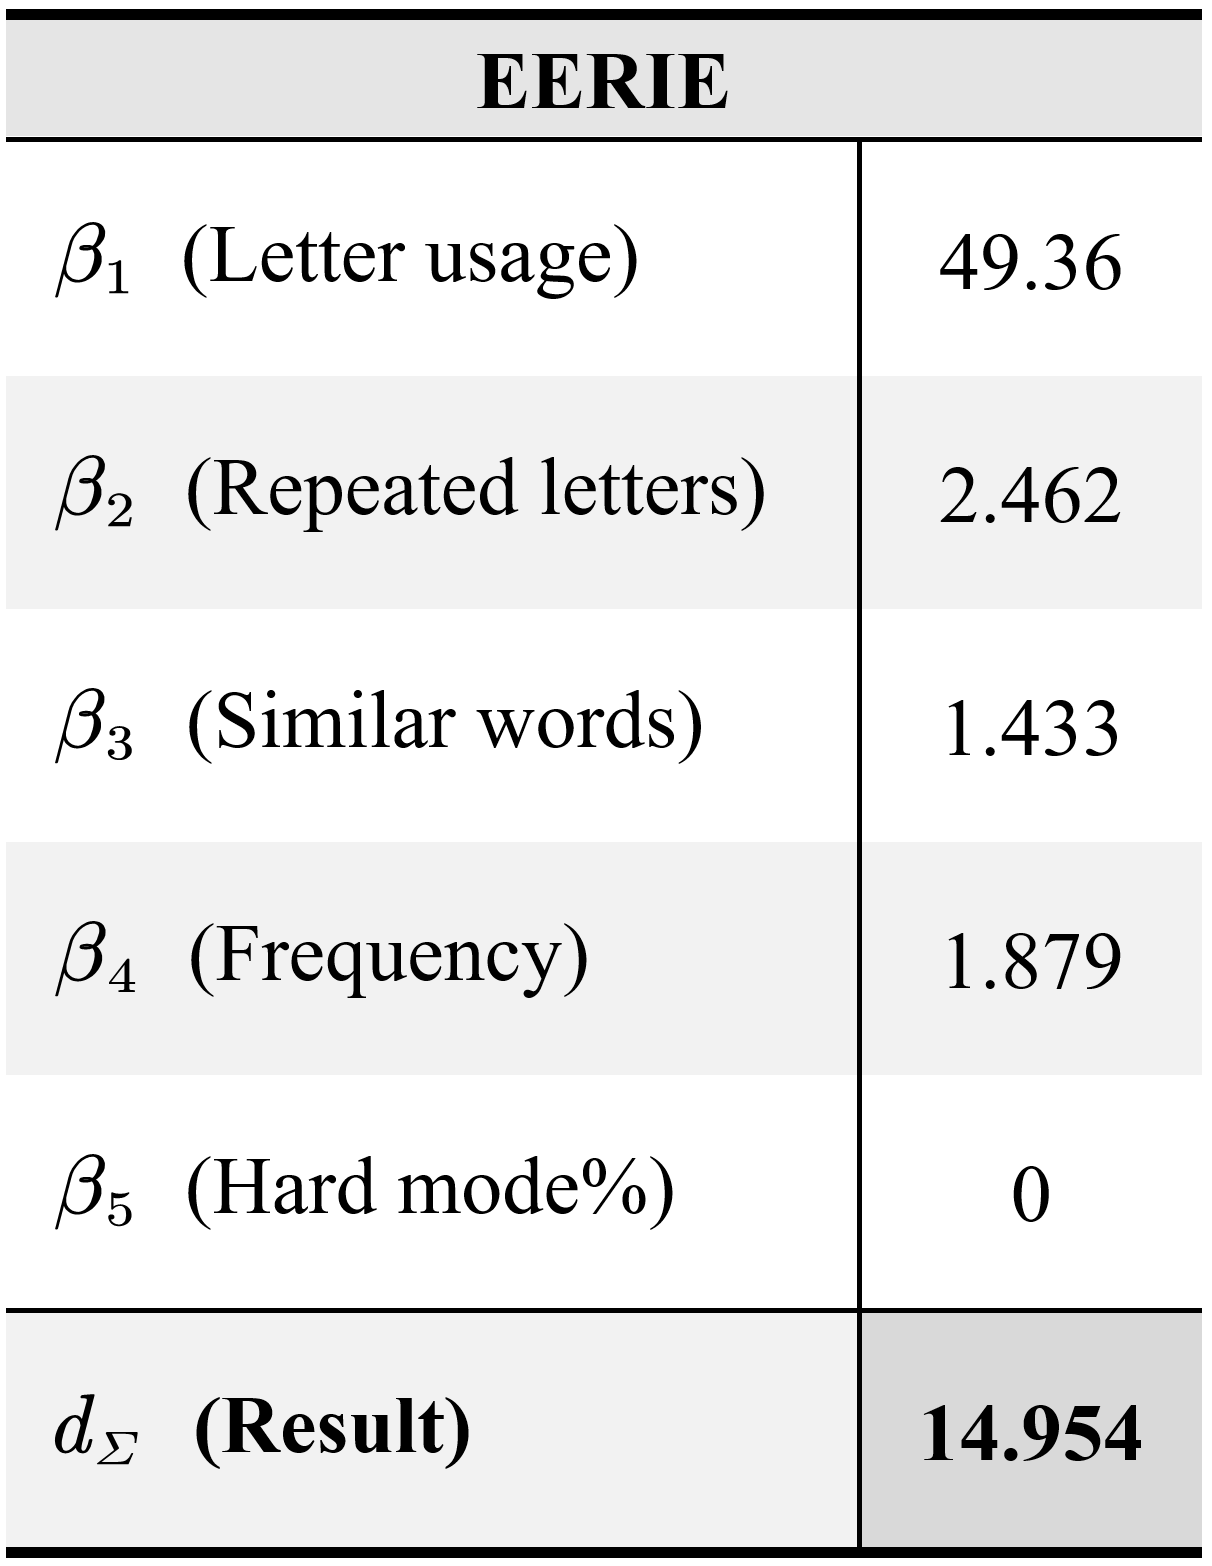
\includegraphics[width=\textwidth]{table7}
		\subcaption{Attributes and difficulties of EERIE}
		\label{fig14_1}
	\end{minipage}
\quad
	\begin{minipage}[c]{0.7\textwidth}
		\centering
		\includegraphics[width=\textwidth]{level}
		\subcaption{Actual versus estimated difficulty level of words}
		\label{fig14_2}
	\end{minipage}
	\caption{Application of Difficulty Evaluation Model and Classification Model}
	\label{fig:14}
\end{figure}

In order to know the difficulty of the word EERIE, we also calculated the values of its various attribute parameters and found its combined difficulty factor $ d_{\varSigma}=14.954 $ (as shown in Figure \ref{fig:14}(a)), which is judged from the classification criteria as a 4-star difficulty word, belonging to the most difficult category.

Observing the Figure \ref{fig:14}(b) and combining the data, we can find that for words with lower difficulty stars, the frequency of use of words or the frequency of use of letters in words are higher. For words with lower difficulty stars, there are more words with repeated letters and words with similar spellings, which can indicate that words in each category have similar properties.
\subsubsection{Analysis of the accuracy of the classification}
\hspace{1.4em}Taking into account the accuracy of the classification and whether the results of the classification are meaningful, we define some evaluation metrics to illustrate the accuracy of the classification model.

Let $ n_{0} $ be the number of words whose prediction result is within the same interval as the actual result, $ n_{1} $ be the number of words whose prediction result differs from the actual result by less than or equal to one star, $ n_{2} $ be the same, and $ n $ be the total number of words predicted.
\begin{table}[!htbp]
	\small
	\centering
	\captionsetup{font={small}} 
	\caption{Accuracy of different definition methods}
	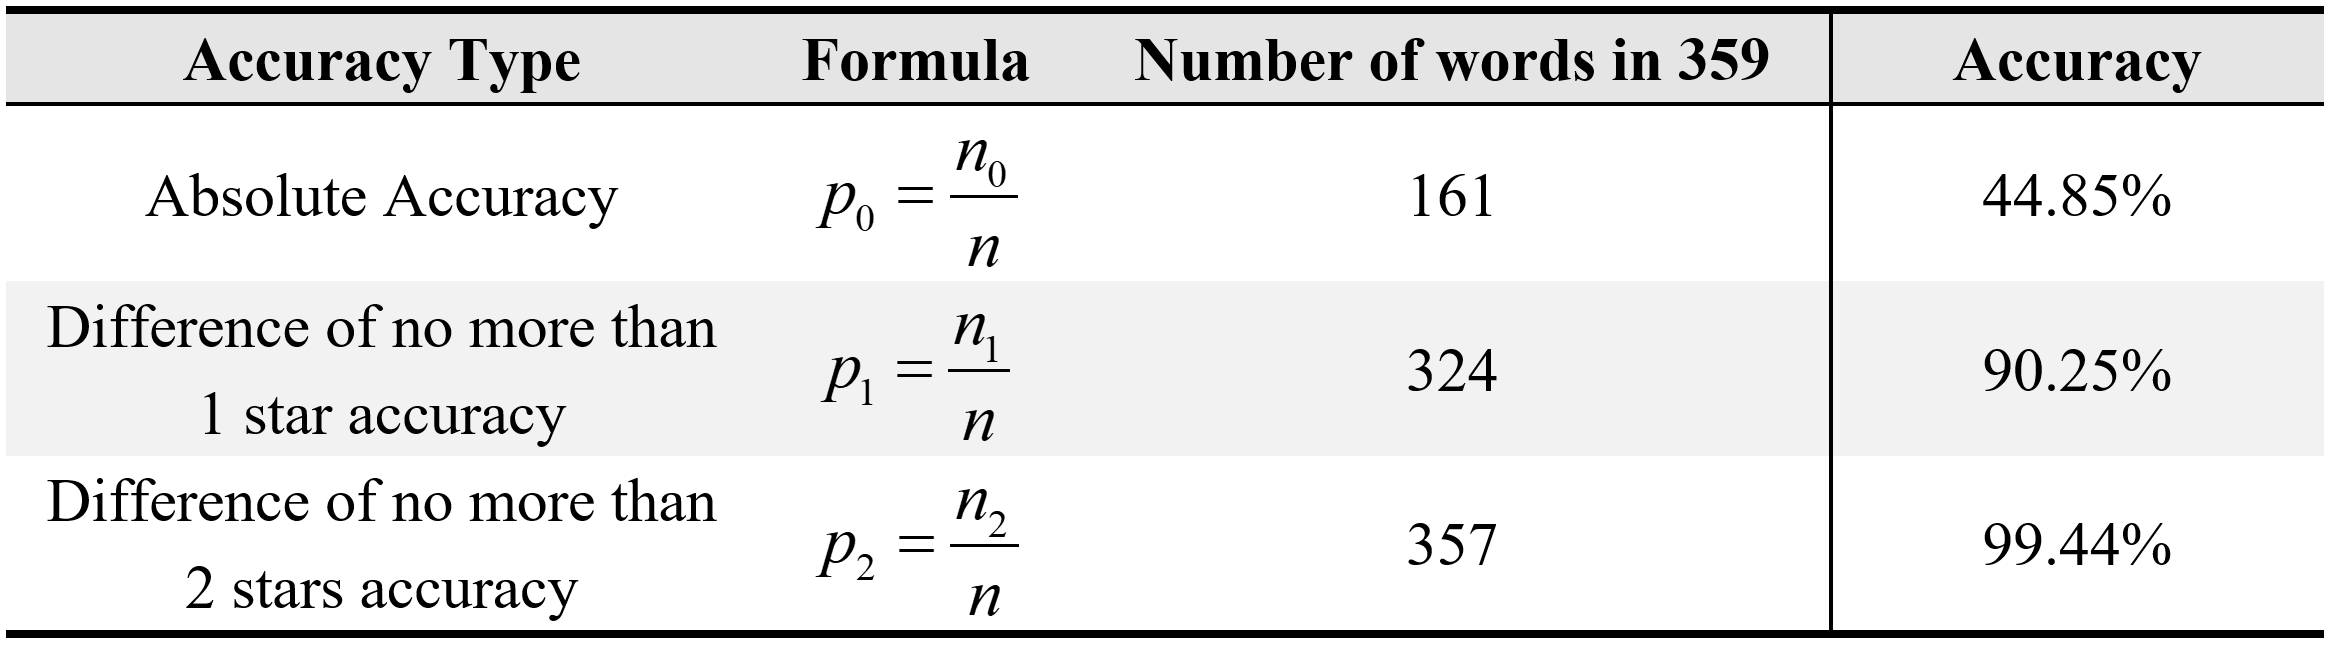
\includegraphics[height=0.23\textwidth]{table8}
	\label{tab:8}
\end{table}
As seen in Table \ref{tab:8}, the difficulty category was judged to be exactly correct for nearly half of the words. And when we allow a 1-star error, the accuracy rate then reaches an amazing 90\%, which indicates that our classification model is accurate.
\\[0.01pt]
\section{Interesting Features of This Data Set}
\hspace{1.4em} In this subsection, the square difficulty factor $ d_{square} $ is used instead of the estimated $ d_{\varSigma} $ because the discussion is about the characteristics of the data set itself.
\subsection{The Feature of Next Day's Hard Mode Percentage}
\hspace{1.4em} In 4.3.2, we noted that the percentage of difficult patterns selected was independent of the characteristics of the solution words on that day. However, we were surprised to find that the percentage of difficult patterns selected on that day seemed to have some negative correlation with the square difficulty factor of the previous day. Thus, we corresponded the daily percentages of the number of difficult choices to the difficulty factors of the previous day, and found the correlation coefficients of the two time series as:

\begin{equation}\label{eq:15}
\rho _{D,P}=\frac{\text{cov}\left( D_{\text{before}},P_{\text{now}} \right)}{\sigma _D\sigma _P}=\frac{E\left[ \left( D-ED \right) \left( P-EP \right) \right]}{\sigma _D\sigma _P}
\end{equation}

where $ D_{\text{before}} $ and $ P_{\text{now}} $ represent two columns of random variables consisting of the square difficulty factor of the previous day and the percentage of hard mode choices for that day, respectively. Solving for the correlation coefficient $ \rho= 0.0495$. Unfortunately, the obtained correlation coefficient does not seem to indicate much of a relationship between the two quantities, or even the opposite of the negative correlation we would expect.

Subsequently, we believe that it may be because the number of people choosing the hard mode is steadily increasing when the wordle is unstable in terms of heat, while the difficulty factor is steady, affecting the judgment of the relationship between the percentage of hard mode and the difficulty of the previous day's word, it may also be because the size of the percentage of hard mode changes less on that day, resulting in a less obvious correlation feature. The hidden rule should actually be: 
\begin{itemize}
	\item when the difficulty factor of the previous day is larger, the difficulty mode percentage of the next day will fall, and vice versa will rise, that is, the difficulty factor of the previous day is negatively correlated with the rate of change of the difficulty mode percentage of the day. As shown in table \ref{tab:6}.
\end{itemize}
\begin{table}[!htbp]
	\small
	\centering
	\captionsetup{font={small}} 
	\caption{Amount of difficulty factor and difficulty percentage change between 12/19 and 12/31 for the previous day}
	\includegraphics[height=0.18\textwidth]{table6}
	\label{tab:6}
\end{table}
We then calculate the correlation coefficient of the two columns of variables in table\ref{tab:6}, at this point $ \rho=-0.432 $. It shows that the difficulty factor of the previous day does have a certain negative correlation with the amount of change in the percentage of difficulty on that day. Combining the data with reality, we can adequately guess that there are some players who, if the difficulty of the word on that day is too high, will not dare to challenge hard mode on the next day, while if the word on that day is too easy, they will choose to challenge hard mode. Since the percentage of challenge hard mode also affects the difficulty factor of the day, we can further guess: 
\begin{itemize}
	\item the change of the difficulty factor of the day is often the opposite of the change of the previous day. That is, the difference between the difficulty factor of each day and the previous day is negatively correlated with the difference between the previous day and the day before that, and such a pattern can also be seen in Figure \ref{fig:11}.
\end{itemize}
\begin{figure}[h]
	\small
	\centering
	\includegraphics[height=0.2\textwidth]{inverse}
	\captionsetup{font={small}}
	\caption{Hard mode percentage change of the day to the previous day's change inverse follow} 
	\label{fig:11}
\end{figure}
Find the correlation coefficient for the two newly constructed columns of variables in Figure \ref{fig:11}, $ \rho=-0.499 $. It can be seen that the two show a strong negative correlation. Of course, there are more reasons than the above for the opposite change in difficulty factors, and there may be other factors such as editor's puzzle-setting rules.
\\[0.01pt]
\subsection{The Feature of One-try}
\hspace{1.4em}We find that when the frequency of words is relatively high, the percentage of one try is often higher, while the opposite is basically 0. This is because people are biased to guess commonly used words when they first guess them.
However, we also find that the percentage of 1 try for high frequency words is also 0. It turns out that this is mainly related to the number of repetitions of letters in the word, i.e. repeated times.
\begin{table}[!htbp]
	\small
	\centering
	\captionsetup{font={small}} 
	\caption{The relationship between the number of letter repetitions in a word and one-try}
	\includegraphics[height=0.16\textwidth]{table9}
	\label{tab:7}
\end{table}

Combining the above data, we can find that when words have repeating letters, even if the words are high-frequency words, the 1 try percentage is biased towards 0. This is well explained by the fact that when playing the wordle game, the first word people guess is always the one without repeating letters, because it tries to line up as many letters as possible and increases the amount of information obtained.
\\[0.01pt]
\section{Test the Model}
\subsection{Sensitivity Analysis of Word Attribute Factor $ \beta_{i} $}
\hspace{1.4em}Using the attribute factors of the word EERIE as a starting point, and choosing the two word-related factors Frequency and Letter score, so that they vary in the following range
$ \beta_{4} $(Frequency)=[640,6640] and $ \beta_{1} $(Letter usage score)=[46.36\%, 52.36\%] to investigate the sensitivity of the difficulty evaluation model to the word attribute factors.

As can be seen from Figure \ref{fig:16}(a), when fixing the other parameter values, the combined difficulty factor $ d_{\varsigma} $ decreases monotonically when Frequency increases and $ d_{\varsigma} $ decreases monotonically when Letter score increases. The results of our model is stable when these two factors are varied within the above interval. Therefore, when there is some deviation in the estimation of Frequency statistic or Letter score, the difficulty does not show much change, which can prove the robustness of our model for these two factors.
\begin{figure}[h]
	\centering
	\captionsetup{font={small}}
	\begin{minipage}[c]{0.5\textwidth}
		\centering
		\includegraphics[width=\textwidth]{heat}
		\subcaption{Sensitivity of the difficulty evaluation model to the frequency of words and usage scores}
		\label{fig16_1}
	\end{minipage}
	\quad
	\begin{minipage}[c]{0.46\textwidth}
		\centering
		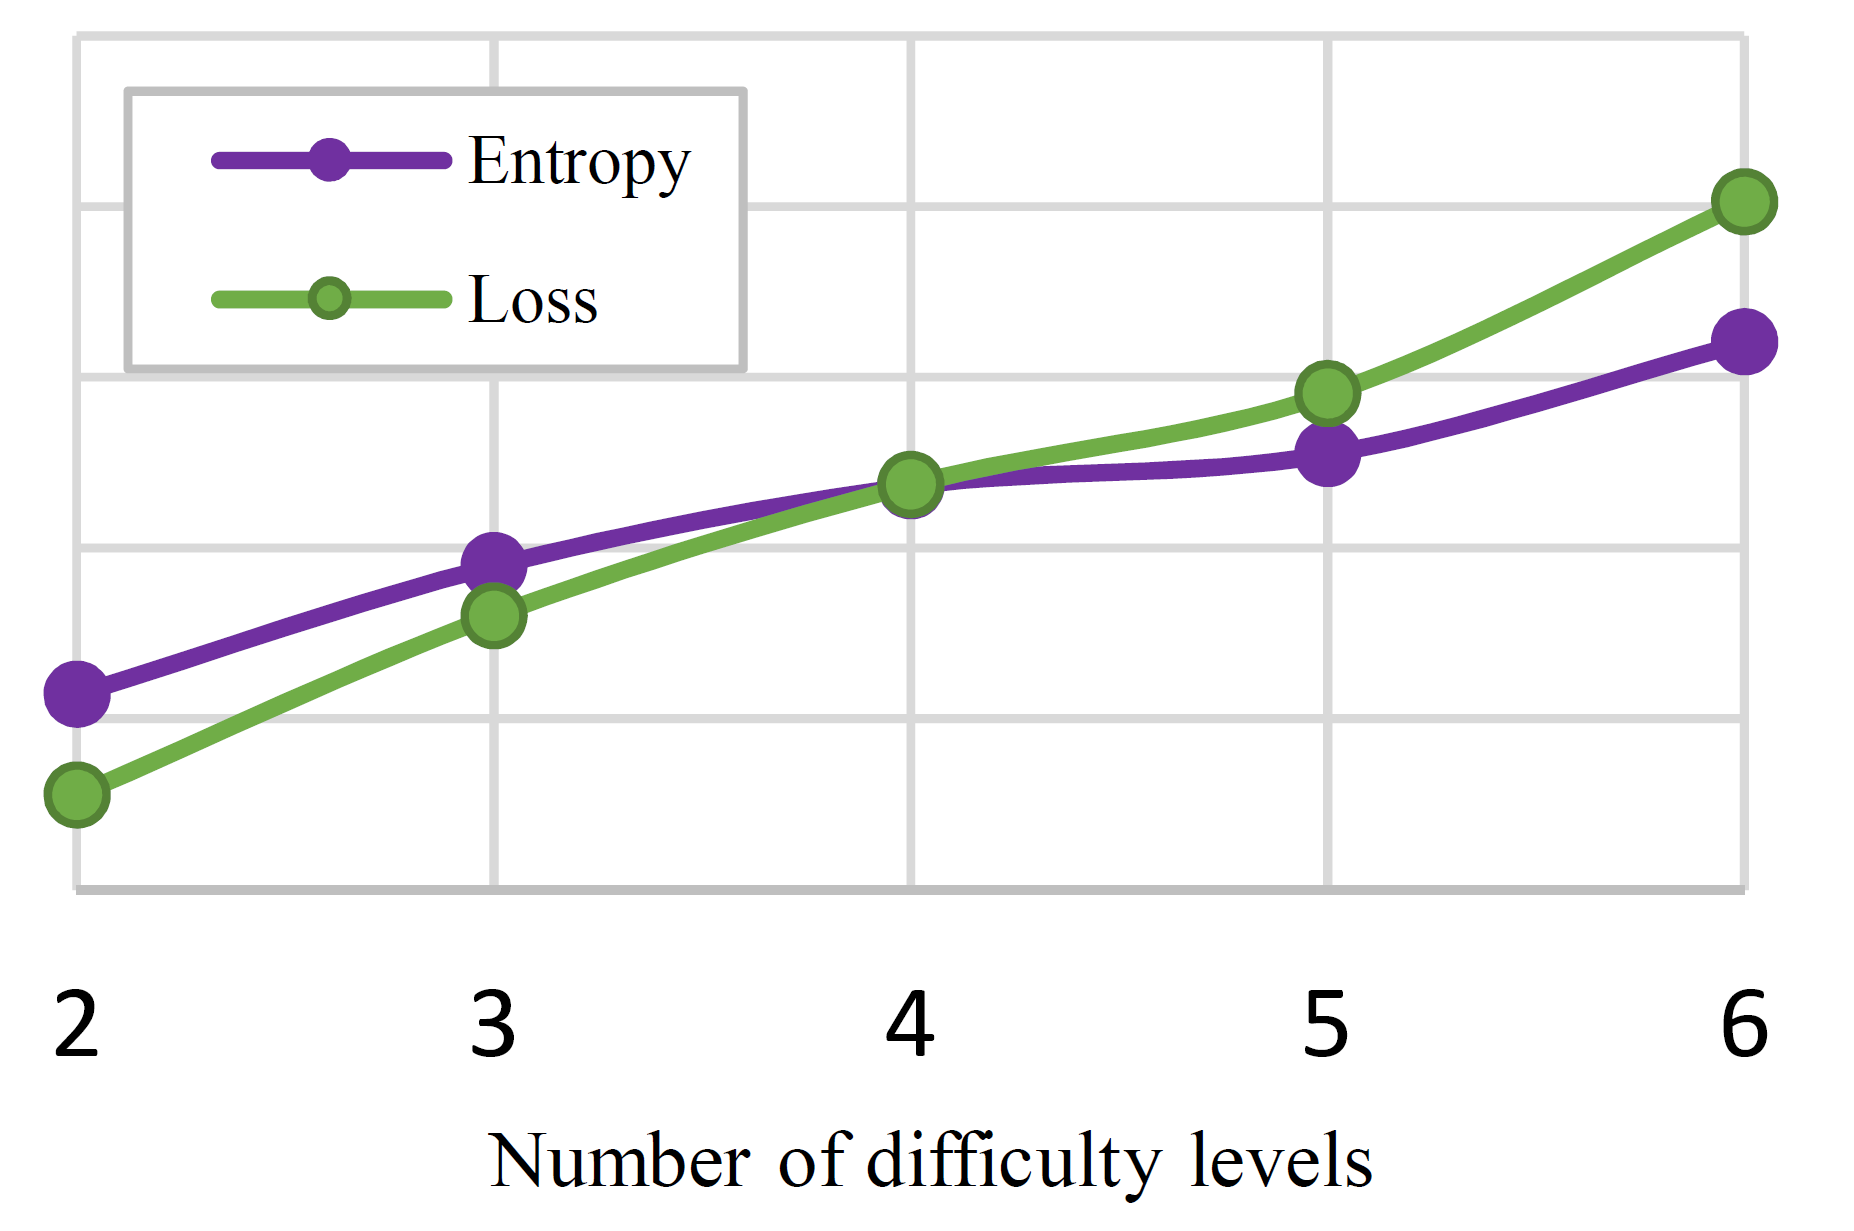
\includegraphics[width=\textwidth]{heat2}
		\subcaption{Sensitivity of the difficulty classification model to the number of classifications}
		\label{fig16_2}
	\end{minipage}
	\caption{Sensitivity analysis of difficulty evaluation models and classification models}
	\label{fig:16}
\end{figure}
\\[0.01pt]
\subsection{Sensitivity Analysis of the Number of Difficulty Classification}
\hspace{1.4em}In the difficulty classification model, the setting of the number of difficulty levels (stars) is very important. The fewer the number of levels, the more words will be classified into the same category and the classification accuracy will be improved, at the same time, the reduction of the number of stars will lead to the reduction of the amount of information contained in the classification, when the classification level is only one star, there is no doubt that all words will be classified accurately, but the classification will become meaningless. We can use information entropy to study the sensitivity of the model to the number of difficulty levels.

\begin{equation}\label{eq:19}
	H(X)=-\sum_{i=1}^n p_i \log p_i
\end{equation}
The Equation \ref{eq:19} is used to measure the amount of information contained in the classification, and the classification accuracy is measured by the loss function used in the optimization of the difficulty classification model. As shown in Figure \ref{fig:16}(b), a difficulty level of 4 is the inflection point of information entropy and loss. Thereafter, the gradient of information entropy decreases and the increase in Loss becomes dramatic. We choose 4 as the number of categories for difficulty classification, which is the best choice to combine both.
\\[0.01pt]
\section{Model Evaluation and Further Discussion}
\subsection{Strengths}
\begin{itemize}
\item In Problem 1, an ARIMA model is applied to predict the time series, and some preprocessing of the data is done to make the resulting model a better fit for the change in the number of participation reports over time.
\item In Problem 2, a coupled double normal distribution model is applied to fit the distribution of the reported results to the normal type distribution observed in the approximate superposition of the data, and a satisfactory result is obtained.
\item In Problem 2,3, not only four word-related factors are introduced, but a word-independent factor error, which is related to the number of people choosing hard mode, is also introduced to optimize the fit of the first four factors to the model.
\end{itemize}
\subsection{Weakness}
\begin{itemize}
	\item Only the four most influential factors are introduced when considering the factors related to word attributes, while other factors with less influence, such as the word's etymological region and word category, are not taken into account, so the model don't achieve a perfect fit to the actual values.
\end{itemize}
\subsection{Possible Improvements}
\hspace{1.4em}\textbf{1)} More complex word attribute factor processing models can be used to optimize the relationship between attributes and word difficulty.

\textbf{2)} The amount of data can be increased to optimize each correlation coefficient and improve the degree of data fit.

\textbf{3)} The accuracy of the data source can be improved. For example, the distribution of the reported results can be more reliable by making the data source accurate to one decimal place.

\textbf{4)} When fitting the distribution of the reported results with a coupled double normal distribution model, it is possible to consider increasing the computational effort by directly using each factor as an input parameter, thus avoiding the error amplification caused by using two models in series.
\includepdf{Letter.pdf} 
\newpage
\begin{thebibliography}{99}
	\bibitem{1}S.L. Ho, M. Xie,The use of ARIMA models for reliability forecasting and analysis,Computers \& Industrial Engineering,Volume 35, Issues 1–2,1998.
	\bibitem{2}Scientific Platform Serving for Statistics Professional 2021. SPSSPRO. (Version 1.0.11)[Online Application Software]. Retrieved from https://www.spsspro.com.
	\bibitem{3}https://en.wikipedia.org/wiki/Letter frequency
	\bibitem{4}https://www.english-corpora.org/coca/
	\bibitem{5}Draper, N.R. and Smith, H. Applied Regression Analysis. Wiley Series in Probability and Statistics. 1998.
\end{thebibliography}
\end{document}

